\label{sec:nueselection:inclusive}


\newcommand{\nueccinc}{$\nu_e$ CC inclusive\xspace}
\newcommand{\nueccsel}{$\nu_e$ CC inclusive selection\xspace}


The aim of the inclusive charged-current electron neutrino selection is to select electron neutrinos independently of their final state and energy. The selection efficiency is approximately 20\%, leading to 250-300 electron neutrino's in the Run 1-4 data-set. The purity without CRT is $\approx 35-40\%$ and with CRT $\approx 45-50\%$.

\subsubsection{Pre-selection}
The selection builds on top of the SliceID (\cref{sec:sliceID}). At the preselection stage,  the cuts listed in \cref{tab:nuecc:presel} are applied. %Here, an electron candidate shower is defined as a particle with a \textit{track\_score} below 0.3, and hits on all three planes. Furthermore, a minimum calorimeric energy of \SI{75}{\MeV} is required. 
\begin{comment}
\begin{table}[h!]
\centering
\setlength{\tabcolsep}{10pt}
\renewcommand{\arraystretch}{1.25}
 \begin{tabular}{| c | c |} 
 \hline
 Cut goal & Cut definition \\
 \hline\hline
Signal topology & An electron candidate shower \\
 \hline
\multirow{2}{*}{Cosmic rejection} & topological\_score $>$ 0.15 \\
 & CosmicIP $>$ $\SI{15}{\cm}$ \\
 \hline
Fiducial volume & \makecell{Reconstructed, space-charge corrected vertex \\ inside a volume defined by borders of \\ \SI{10}{\cm} in $x$ and $y$ and $[ \SI{20}{\cm}, \SI{50}{\cm}]$ in $z$} \\
 \hline
Reconstruction quality & \textit{slclustfrac} $>$ 0.4 \\
\hline
Electron Candidate &  track\_score $<$ 0.3, hits in all three planes \\
\hline
Michel rejection & shr\_energy\_tot\_cali $>$ 0.075 GeV \\
 \hline
 \end{tabular}
 \caption{\label{tab:nuecc:presel} Preselection requirements for the \nueccsel.  }
\end{table}
\end{comment}
At this stage, the efficiency of the selection is 46\% for $\nu_e$ CC events inside the fiducial volume\textcolor{blue}{Do we have the plot of efficiency as a function of true nu E? }. This is equivalent to 618 events per \SI{10.1e20}{POT}. The number of LEE signal events passing is approximately 30 per \SI{10.1e20}{POT}. The purity at this stage is $\sim$3.0\%. 

After the pre-selection cuts, the $\nu_e$ CC purity is still low. Figure \ref{fig:pre_shower_E_pdg} shows the distribution of the angles of the electron candidate shower highlighting the dominant background categories: the main background is coming from events with $\pi^0$ in the final state. Thus, $e/\gamma$ separation becomes key to the $\nu_e$ CC inclusive selection.

\cref{fig:e_cand_Calo} shows the agreement in the kinematics of the electron candidate shower at the preselection stage. \emph{As seen in several other Data-MC comparisons of calorimetry variables throughout this note, a slight disagreement is found in the shower candidate energy, to be re-evaluated after the planned MC re-calibration.}


\begin{figure}[h]
    \centering
    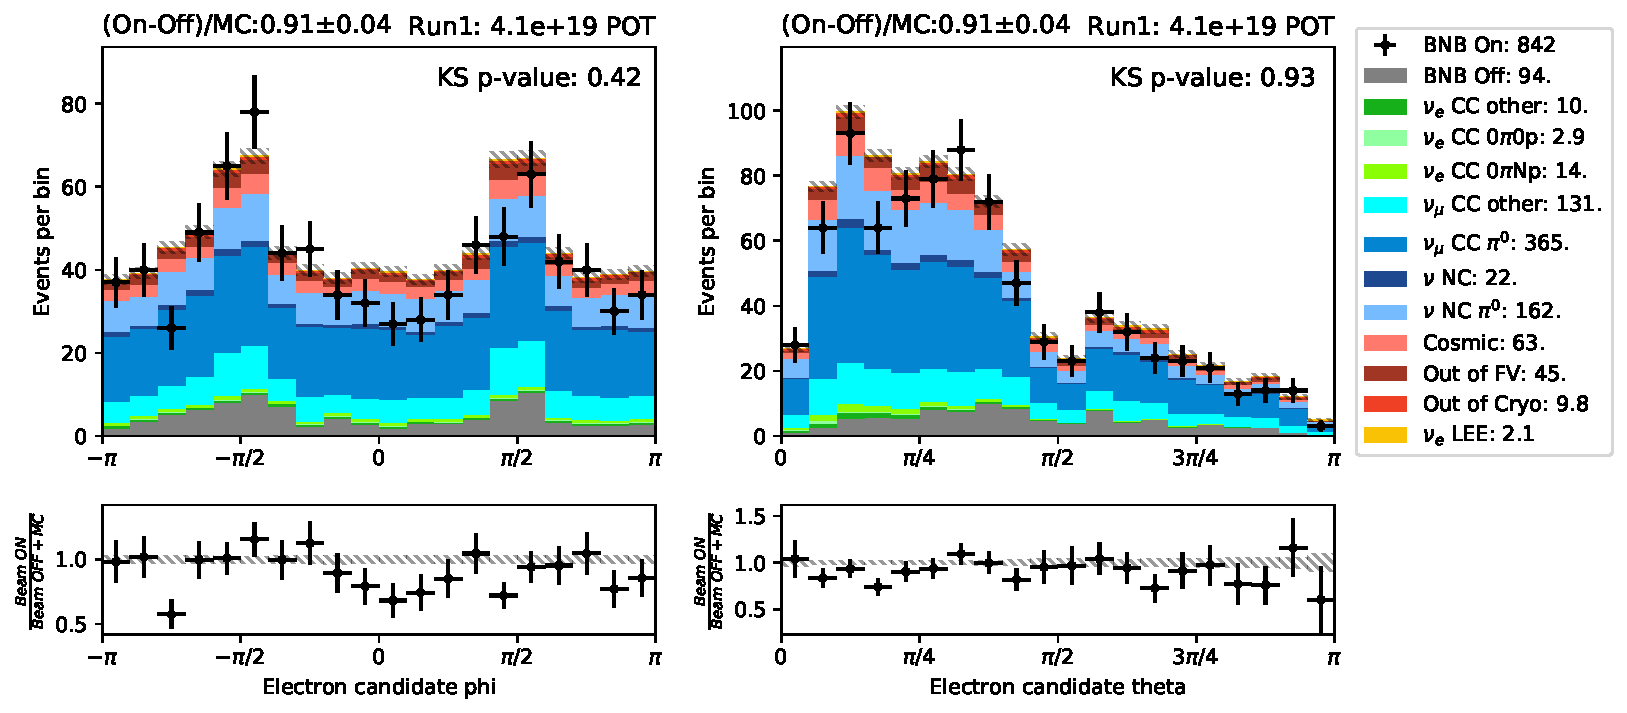
\includegraphics[height=4.9cm]{NueCCsel/Images/run1/pre_angles.pdf}
    \caption{MC-Data comparison of the angles of the electron candidate after the pre-selection cuts.}
    \label{fig:pre_shower_E_pdg}
\end{figure}

\begin{figure}[h]
    \centering
     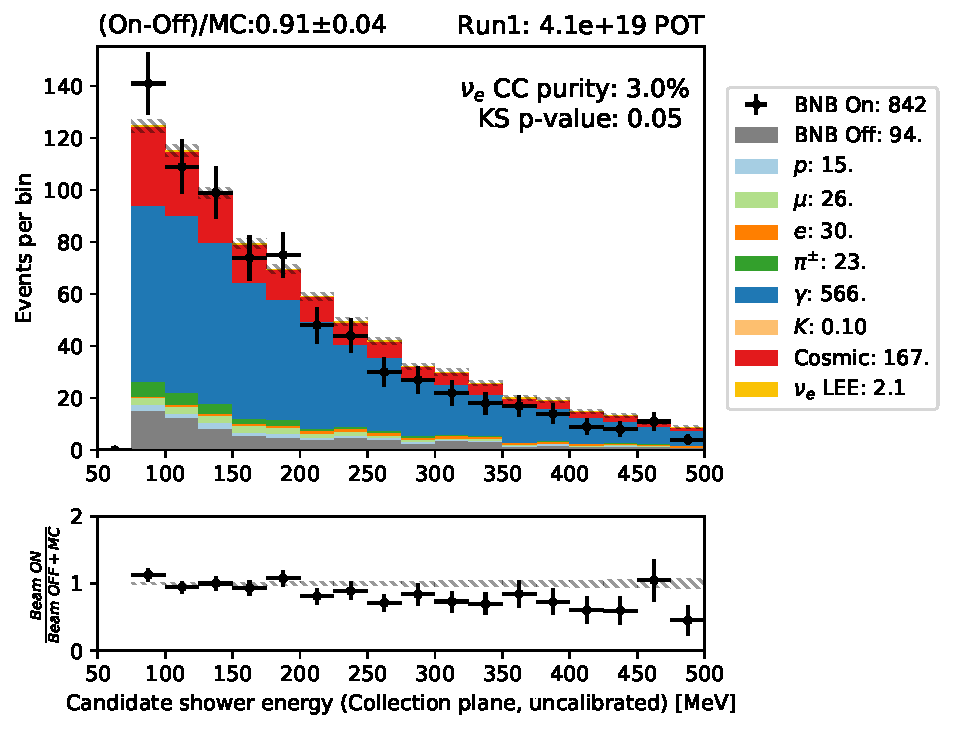
\includegraphics[height=4.9cm]{NueCCsel/Images/run1/pre_shower_E_pdg.pdf}
    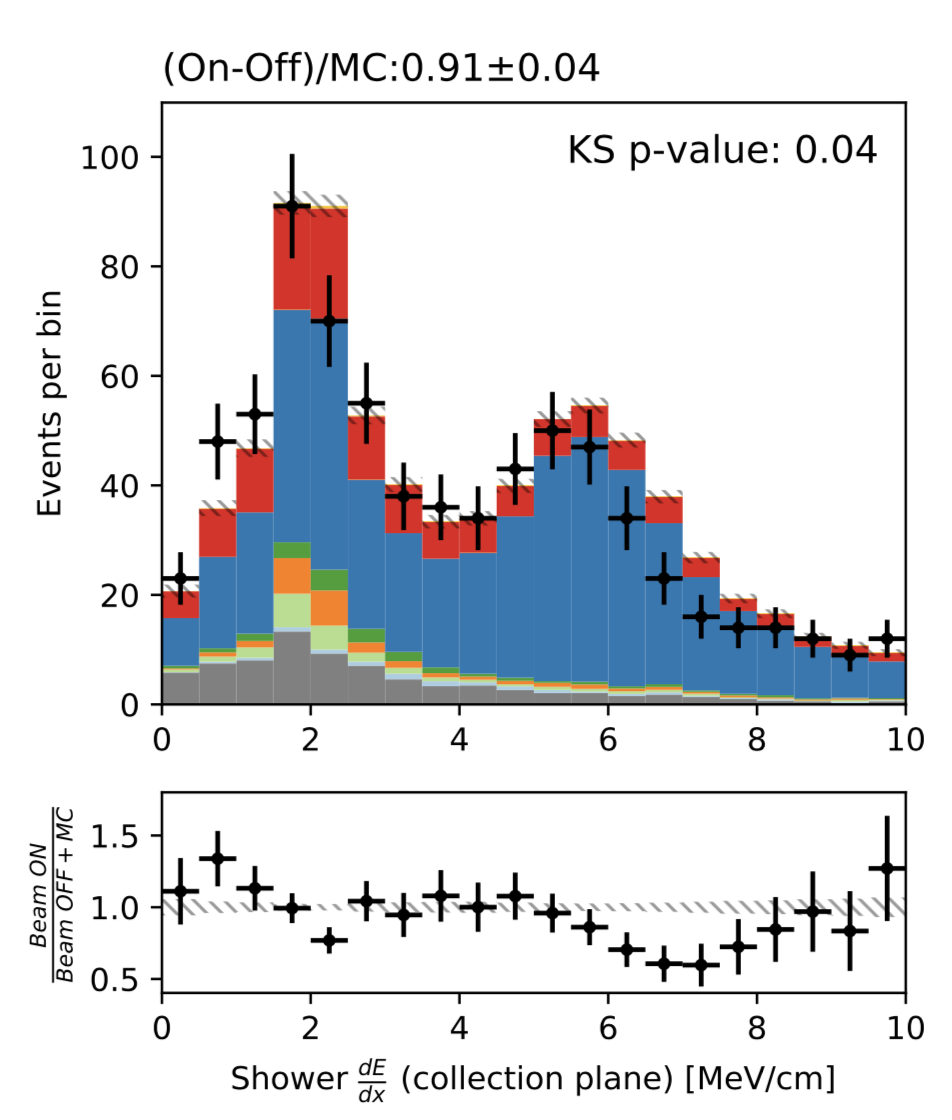
\includegraphics[height=4.9cm]{NueCCsel/Images/run1/e_cand_dedxColl}
    \caption{ Energy (\emph{Left}) of the electron candidate after the pre-selection cut d$E$/d$x$ on the collection plane (\emph{Right}) of the electron candidate shower after the pre-selection.}
    \label{fig:e_cand_Calo}
\end{figure}


\subsubsection{Electron Identification}
After the pre-selection, the object that is tagged as electron candidate is still not an neutrino electron in the dominant fraction of events. The ratio photons to electrons is approximately 20 to 1 and photon-electron separation is therefore the main objective of electron identification. The identification is done using a boosted decision tree, trained on variables characterizing the particle. 

Even if a number of variables contribute to the BDT (see backup \ref{sec:datamc:nueccinclusive}),  we highlight here some distributions which show the cleanest e/$\gamma$: separation: the  d$E$/d$x$ distribution on  collection plane (left side of Figures \ref{fig:e_cand_Calo}), the shower vertex distance and average molier radius (\cref{fig:e_cand_dist} left and center) . The response of the BDT is shown in the right panel of \cref{fig:e_cand_dist}. The complete list of variables used to train the BDT for electron identification is: \emph{shower\_vtx\_dist}, \emph{nObjHits\_Y},  \emph{shr\_tkfit\_2cm\_dedx\_Y},  \emph{shr\_tkfit\_2cm\_dedx\_ALL},  \emph{shr\_tkfit\_gap10\_dedx\_Y}, \emph{shrmoliereavg}, \emph{secondshower\_Y\_vtxdist}, \emph{subcluster}, \emph{ismerged}.

\begin{comment}
 Those variables are listed in \cref{tab:nuecc:e_bdt}.

\begin{table}[h!]
\centering
\setlength{\tabcolsep}{10pt}
\renewcommand{\arraystretch}{1.25}
\begin{tabular}{| c | c |} 
\hline
Cut goal & Cut definition \\
\hline\hline
\multirow{2}{*}{$e/\gamma$ separation} & Shower vertex distance \\
                                       & \makecell{Shower d$E$/d$x$ at the start of the shower: \\
                                            \tabitem On the collection plane only.\\
                                            \tabitem Weighted mean over the 3 planes.\\
                                            \tabitem Collection plane, but shifted by \SI{1}{\cm}.\\ 
                                            }\\
\hline
\multirow{2}{*}{$\pi^0$ tagging} & \textit{secondshower\_Y\_nhit} \\
 & \textit{secondshower\_Y\_vtxdist} \\
 \hline
\multirow{2}{*}{$\mu$-rejection} & \textit{shrmoliereavg} \\
                                 & \textit{subcluster} \\
 \hline
Reconstruction quality & \makecell{\textit{ismerged} \\ Checks if a proton is merged in the start of the shower. } \\
 \hline
 \end{tabular}
 \caption{\label{tab:nuecc:e_bdt} Input variables used by the BDT to do electron identification.}
\end{table}
\end{comment}


\begin{figure}[h]
    \centering
    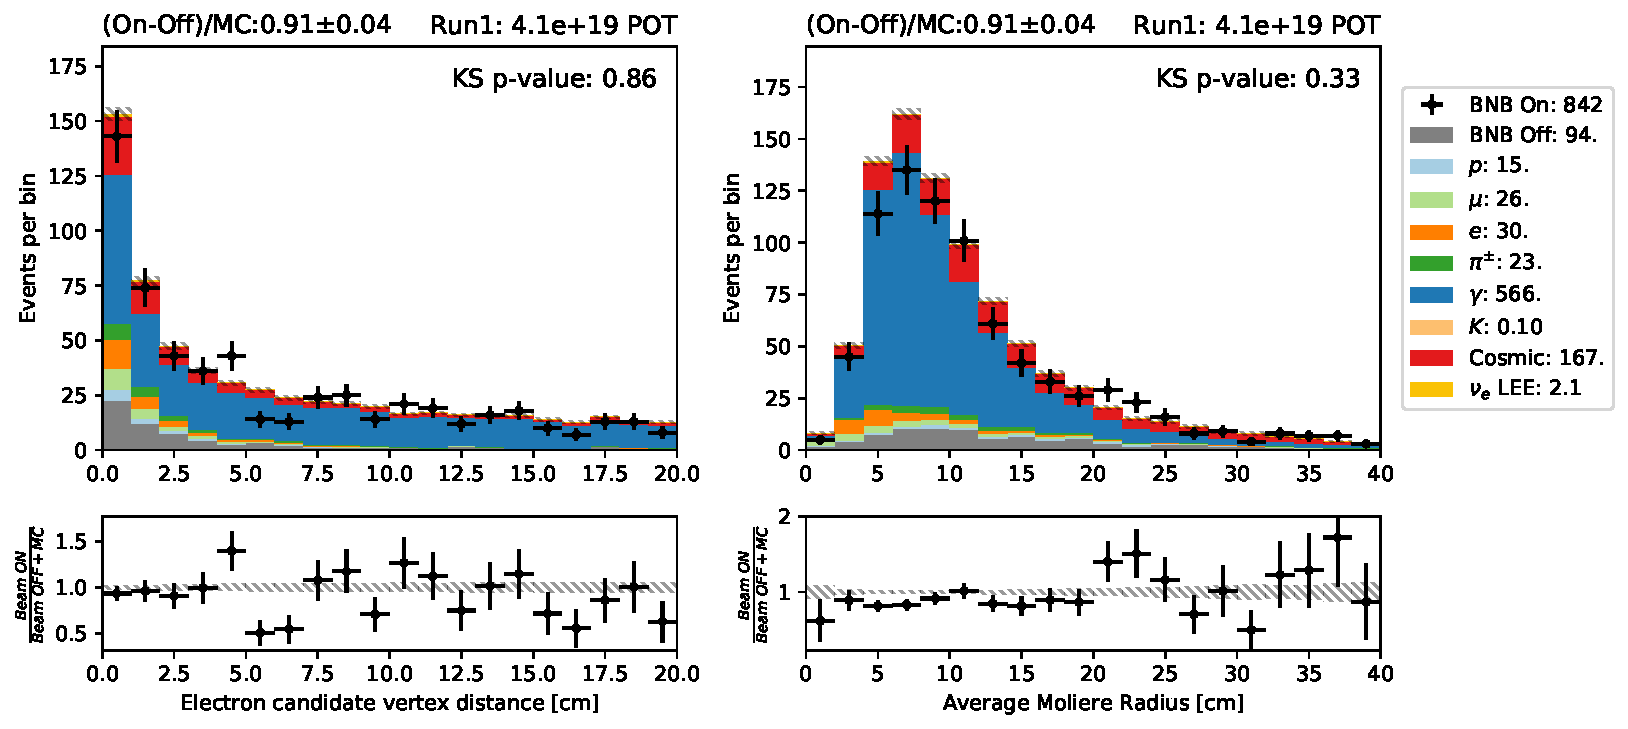
\includegraphics[height=5cm]{NueCCsel/Images/run1/e_cand_dist.pdf}
    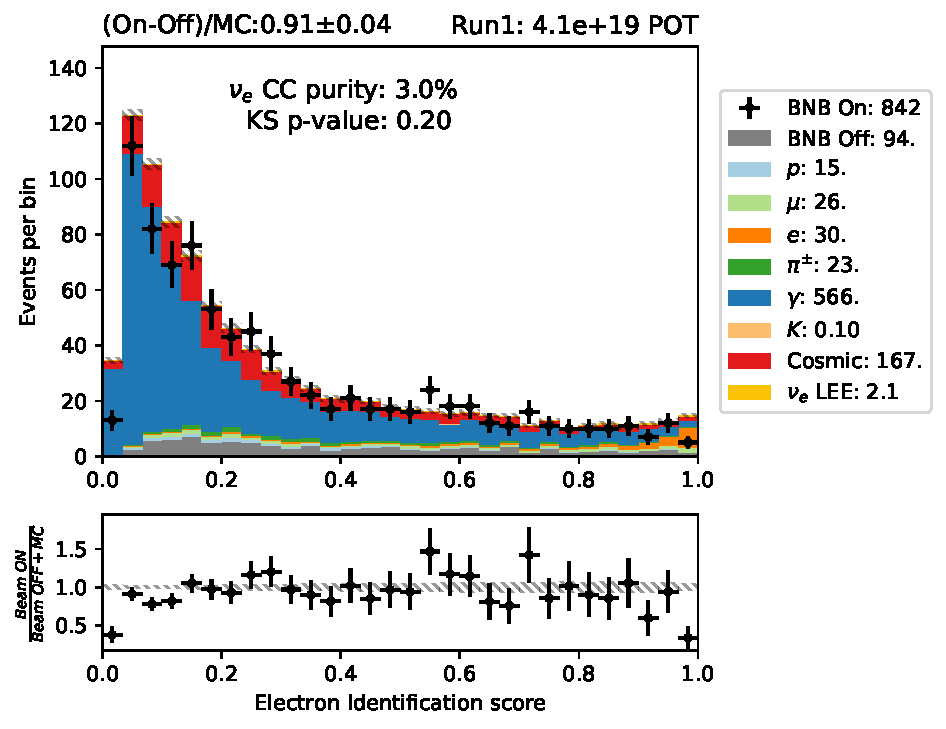
\includegraphics[height=5cm]{NueCCsel/Images/run1/pre_e_score.pdf}
    \caption{The left two panels show important variables to identify electrons after the pre-selection. The right panel shows the BDT electron identification response, demonstrating a good e/$\gamma$ separation.}
    \label{fig:e_cand_dist}
\end{figure}

%\begin{figure}
%    \centering
%    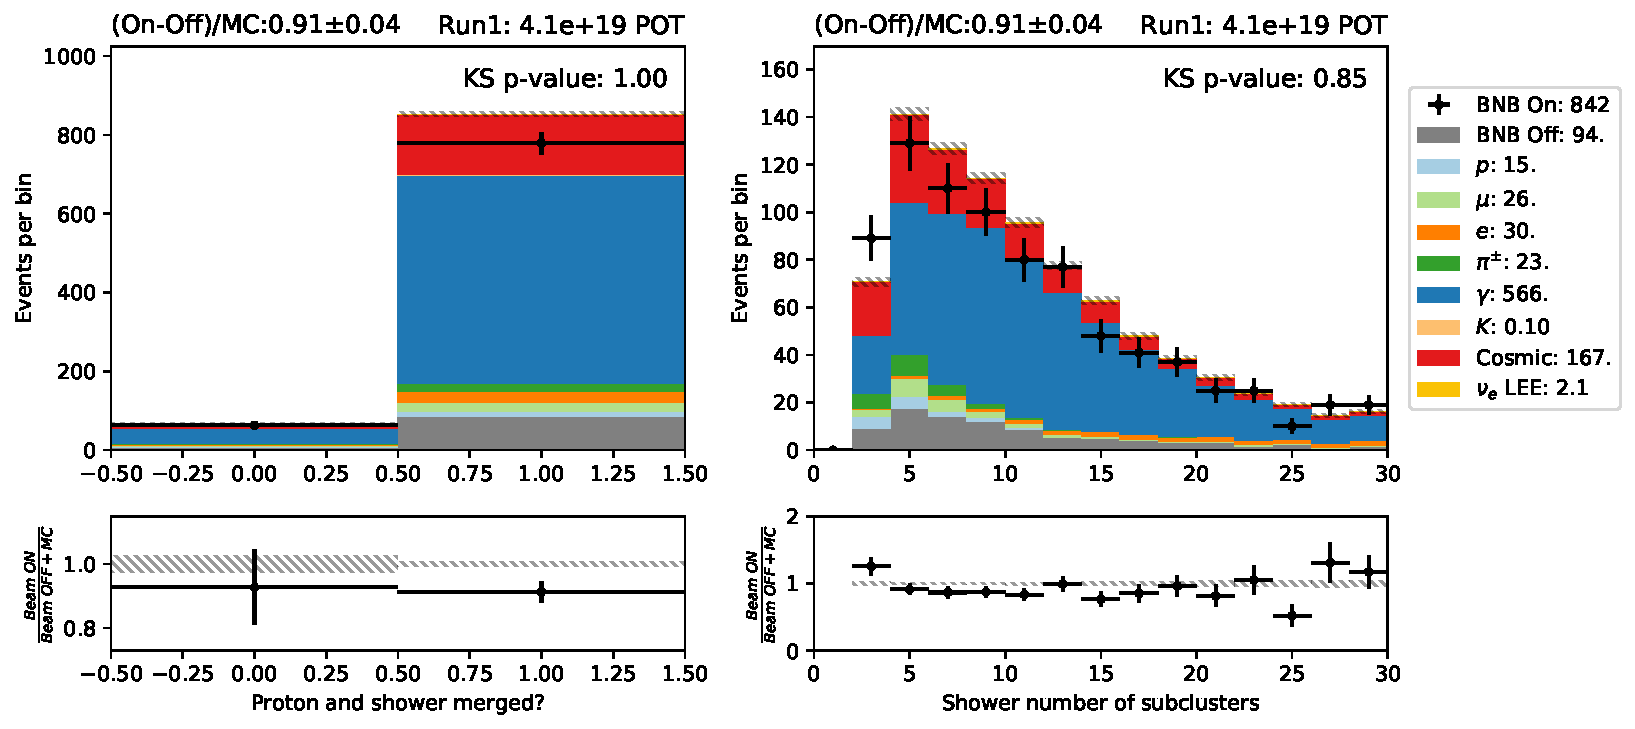
\includegraphics[width=\textwidth]{NueCCsel/Images/run1/e_cand_subclusters.pdf}
%    \caption{Caption}
%    \label{fig:e_cand_subclusters}
%\end{figure}

%\begin{figure}
%    \centering
%   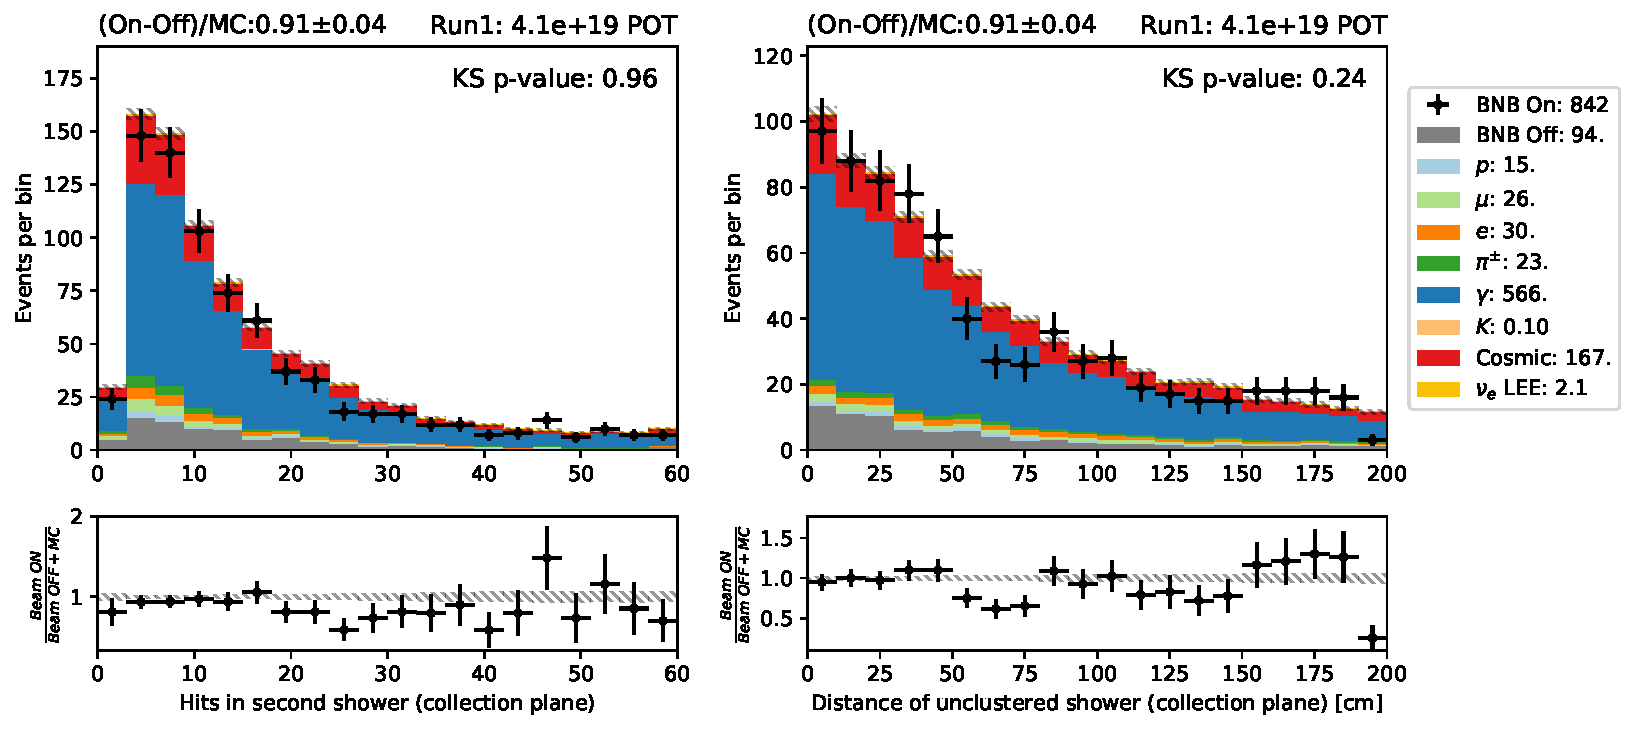
\includegraphics[width=\textwidth]{NueCCsel/Images/run1/e_cand_secondshower.pdf}
%    \caption{Caption}
%    \label{fig:e_cand_secondshower}
%\end{figure}

\subsubsection{Other Daughters Identification}
A number of particles are present in the slice besides the electron candidate. We leverage those PFParticles to improve background rejection. We train a BDT on PFParticles divided in two categories:
\begin{enumerate}
    \item particles backtracked to a proton or a split-off part of the electron;
    \item particles backtracked to a simulated muon or cosmic activity. 
\end{enumerate}
We want to reject events which contain a particle which is overlay or muon like. On the other hand, particles that are backtracked to protons or electron bits are allowed and should not lead to the rejection of the event.
\par The more complicated situation arises when pions are present. Charged pions should be allowed in a $\nu_e$ CC search, but the mis-identification rate between charged pions and muons is large in this detector type. Photons coming from neutral pions, apart of the electron shower candidate, can be part of the $\nu_e$ CC event, but can also help to reduce the NC $\pi^0$ backgrounds. It was chosen therefore to give them a neutral label. 

The input variables of the BDT are listed in \cref{tab:nuecc:other_bdt}



\begin{table}[h!]
\centering
\setlength{\tabcolsep}{10pt}
\renewcommand{\arraystretch}{1.25}
\begin{tabular}{| c | c |} 
\hline
Cut goal & Cut definition \\
\hline\hline
\multirow{3}{*}{particle identification} & \textit{trk\_llr\_pid\_score} \\
                                         & \textit{trk\_distance} \\
                                         & \textit{trk\_score}\\
\hline
\multirow{2}{*}{particle hierarchy} & \textit{pfp\_generation} \\
                                    & \textit{Number of daughters of the particle} \\

 \hline
 \end{tabular}
 \caption{\label{tab:nuecc:other_bdt} Input variables used by the BDT to classify the other daughter particles.}
\end{table}

The three most important distributions of the variables used are given in \cref{fig:pre_daughter_1}. The response of the BDT is shown in \cref{fig:pre_daughter_score}.


\begin{figure}
    \centering
    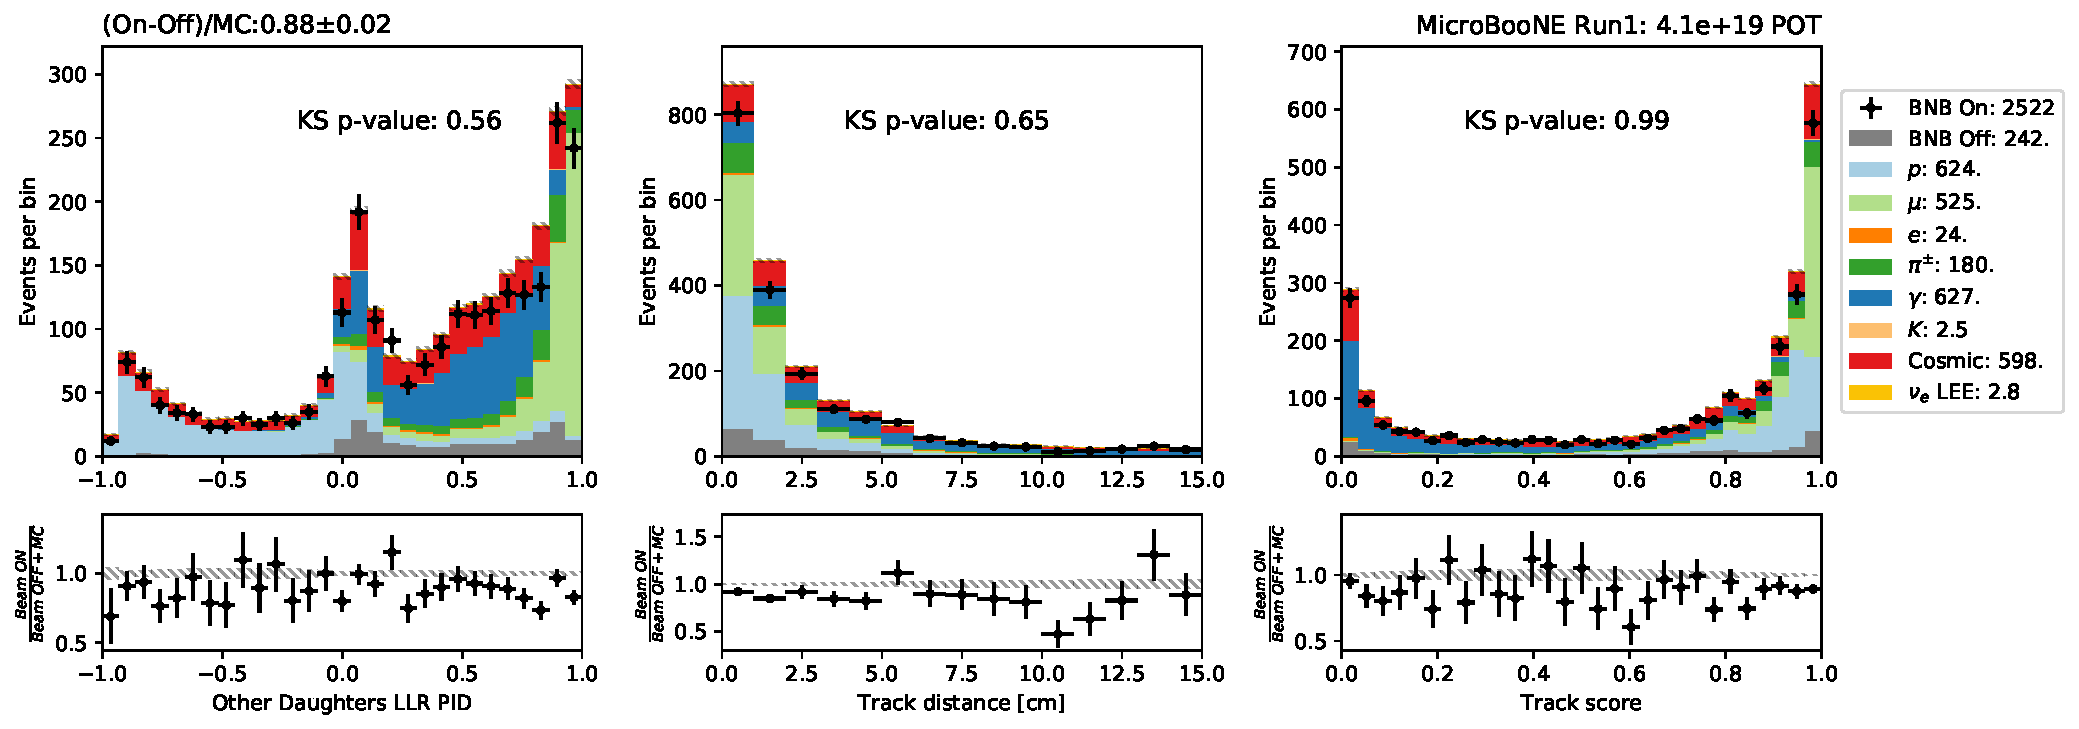
\includegraphics[width=\textwidth]{NueCCsel/Images/run1/pre_daughter_1.pdf}
    \caption{Variables used to identify the other daughters of the neutrino besides the electron candidate shower. The distributions include all non-electron tagged daughters after the pre-selection.}
    \label{fig:pre_daughter_1}
\end{figure}

%\begin{figure}
%    \centering
%    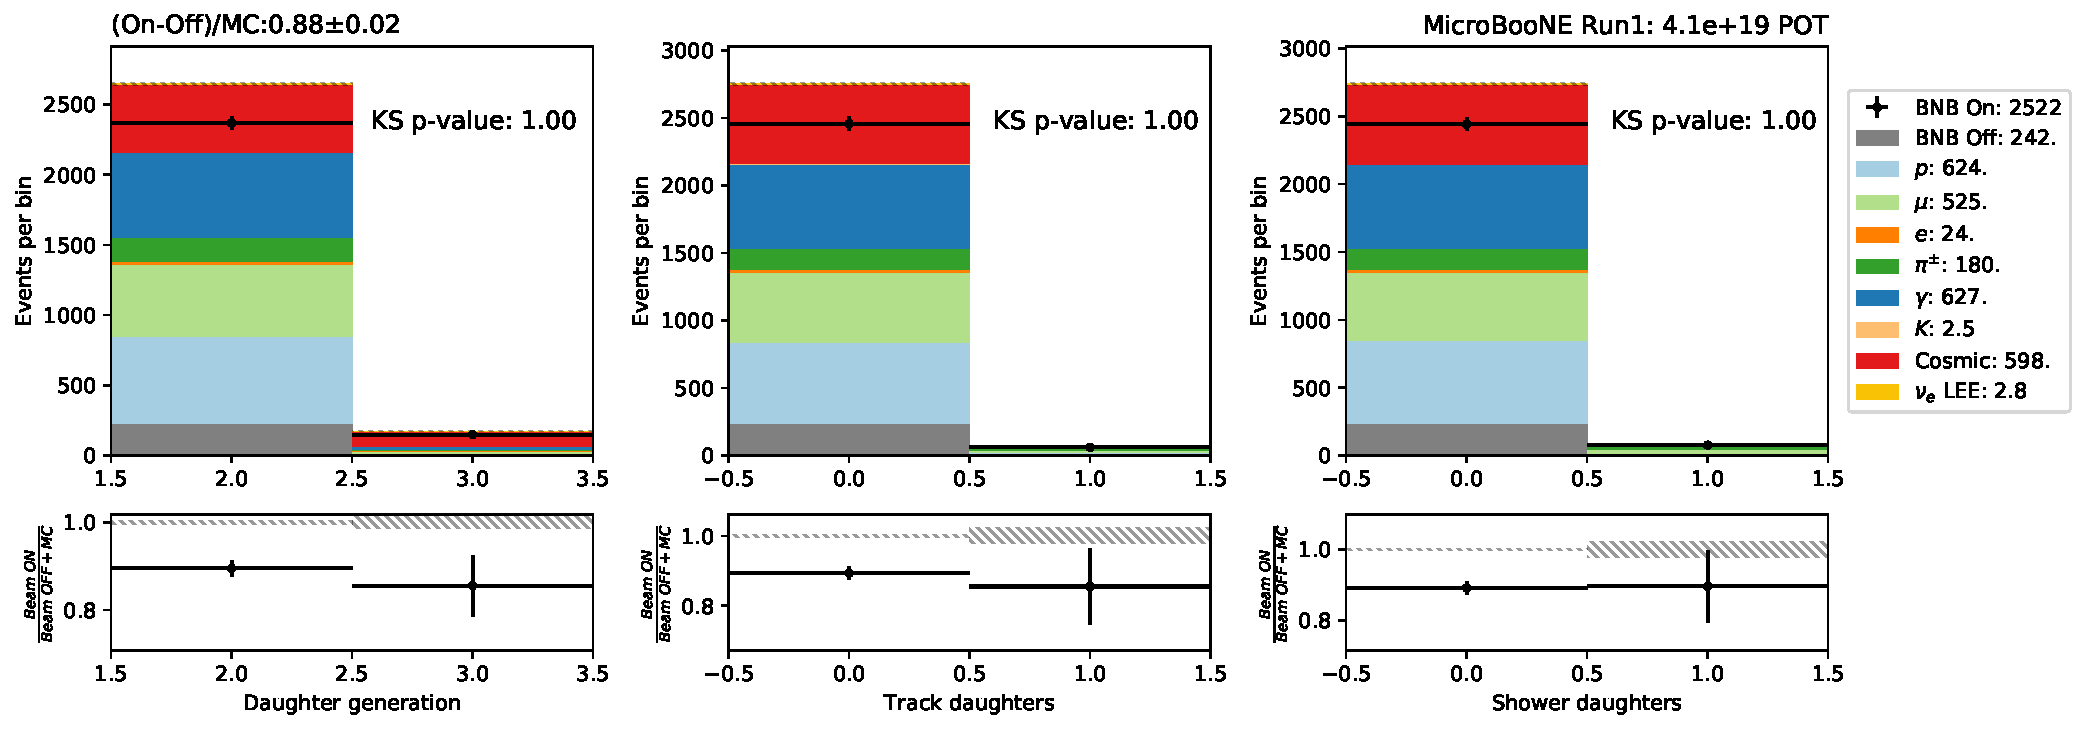
\includegraphics[width=\textwidth]{NueCCsel/Images/run1/pre_daughter_2.pdf}
%    \caption{Caption}
%    \label{fig:pre_daughter_2}
%\end{figure}

\begin{figure}
    \centering
    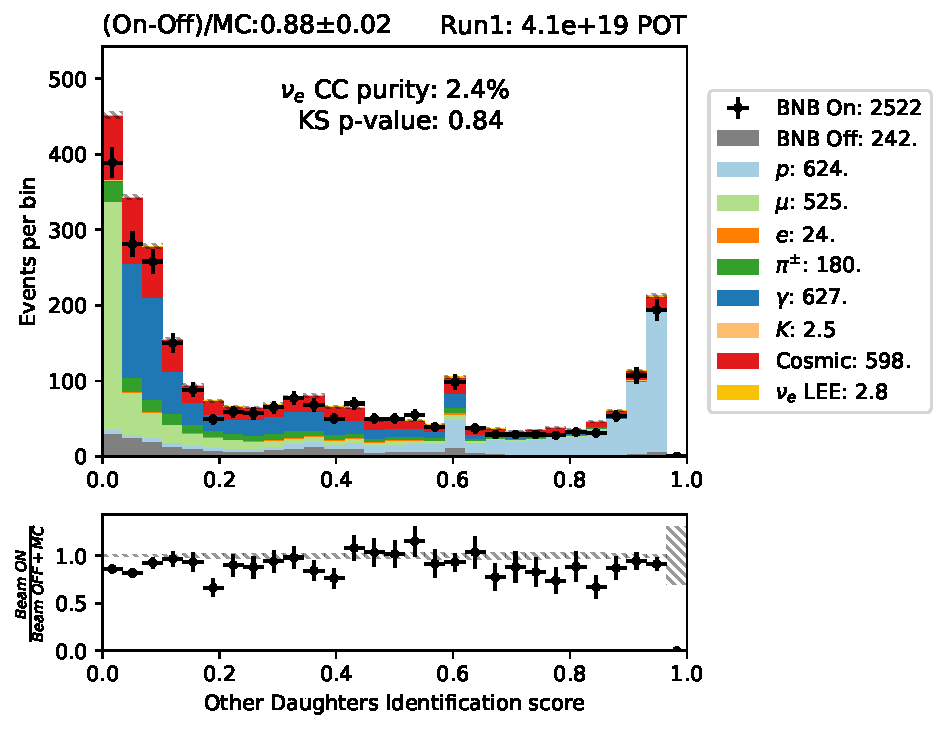
\includegraphics[width=0.5\textwidth]{NueCCsel/Images/run1/pre_daughter_score.pdf}
    \caption{BDT response to classify the non-electron candidate daughters in the event. The cosmogenic particles, together with the muons and photons have a low response, indicating higher likeliness to be background. The protons have a high response on the right.}
    \label{fig:pre_daughter_score}
\end{figure}

\subsubsection{Event Selection}
The final event classification build on top of the particle identification performed in the two previous sections. THe dominating variable is the electron identification response but the full list of variables is, in sequence of importance:

\begin{enumerate}
    \item Electron BDT response
    \item Lowest BDT response of the other daughter BDT from the collection of PFParticles, except the electron candidate shower. In the case of a single shower event, this field is assigned the default value 1. 
    %\textcolor{blue}{(David) Lowest means the score for the least nue-like PFParticle? What happens if no additional PFParticle is present?}
    \item contained\_fraction
    \item Number of showers
    \item hits\_ratio
    \item Mean BDT response of the other daughter BDT from the collection of PFParticles, except the electron candidate shower. In the case of a single shower event, this field is assigned the default value 1. 
    \item Number of particles in the slice that have a reconstructed start point more than \SI{3}{\cm} from the neutrino vertex.
\end{enumerate}
The response of the event classification is given in the left panel \cref{fig:pre_event_score}. After the selection, the efficiency is 21\%, corresponding to 280 electron neutrino's in the Run 1-4 data-set. The distribution of the reconstructed electron energy is given in the right panel of \cref{fig:pre_event_score}. \cref{fig:nueccinc_eff} documents the efficiency of the SliceID, pre-selection and final inclusive selection for the three final state categories.

%\begin{figure}
%    \centering
%    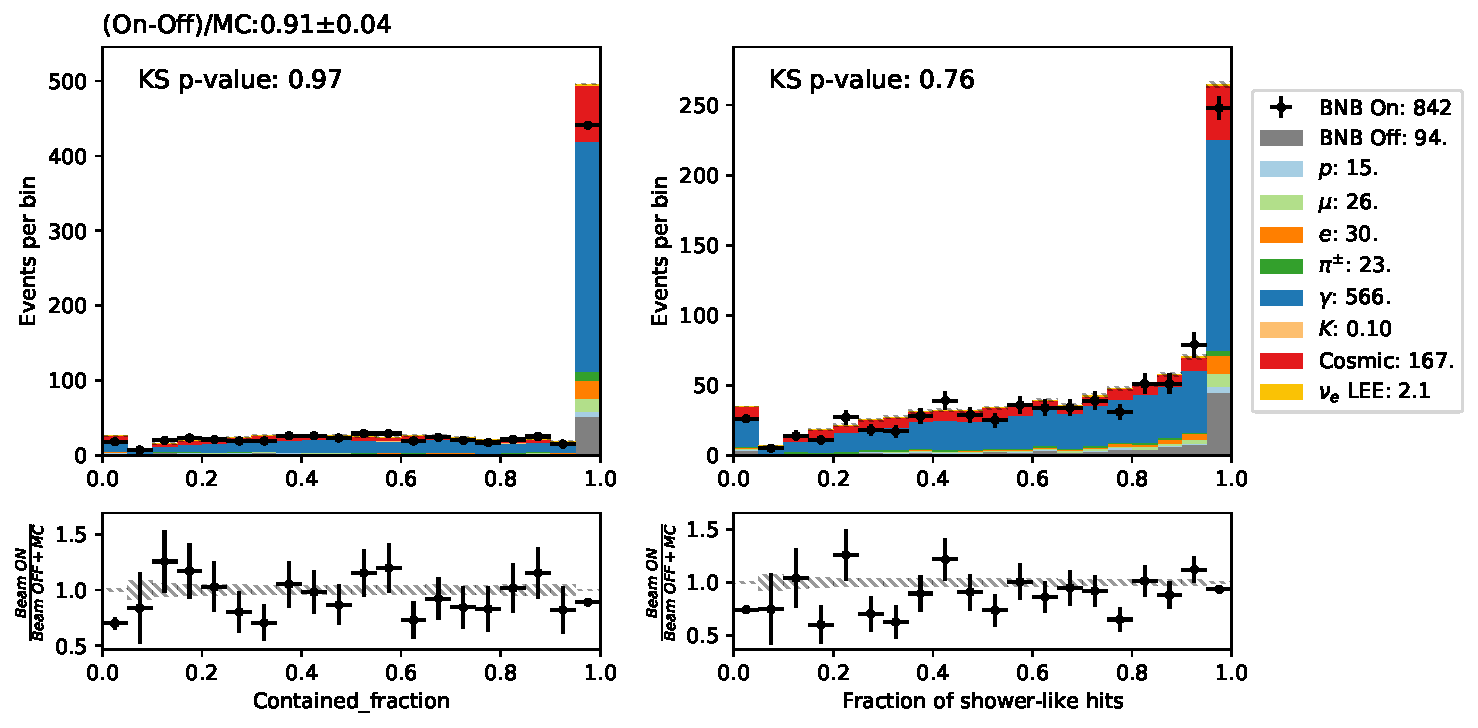
\includegraphics[width=\textwidth]{NueCCsel/Images/run1/bdt_1.pdf}
%    \caption{Caption}
%    \label{fig:bdt_1}
%\end{figure}

%\begin{figure}
%    \centering
%    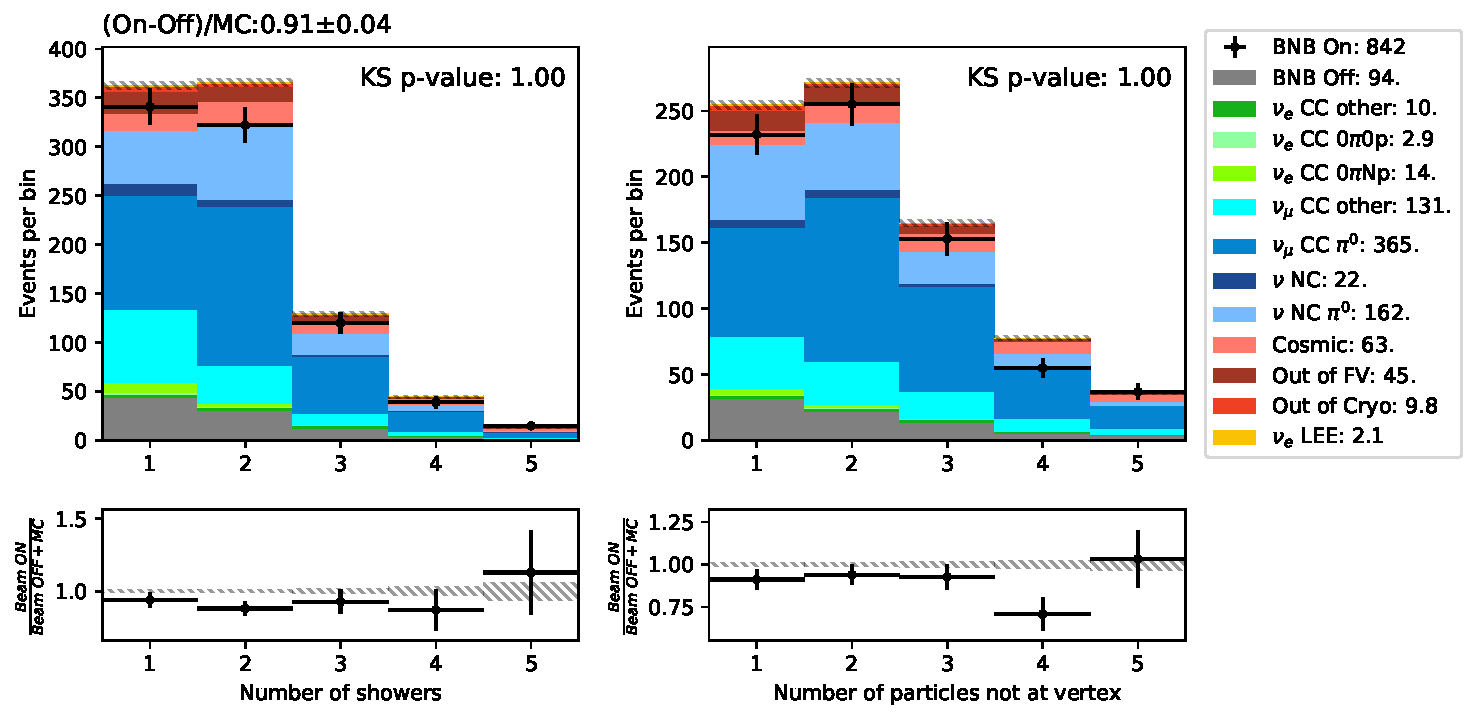
\includegraphics[width=\textwidth]{NueCCsel/Images/run1/bdt_2.pdf}
%    \caption{Caption}
%    \label{fig:bdt_2}
%\end{figure}

\begin{figure}
    \centering
    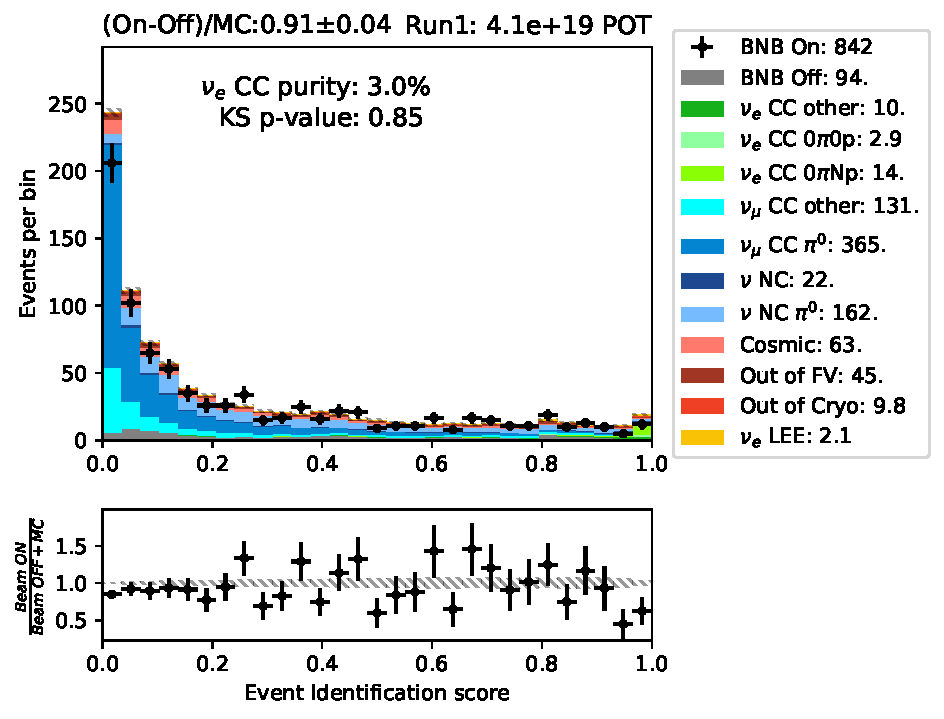
\includegraphics[width=0.445\textwidth]{NueCCsel/Images/run1/pre_event_score.pdf}
    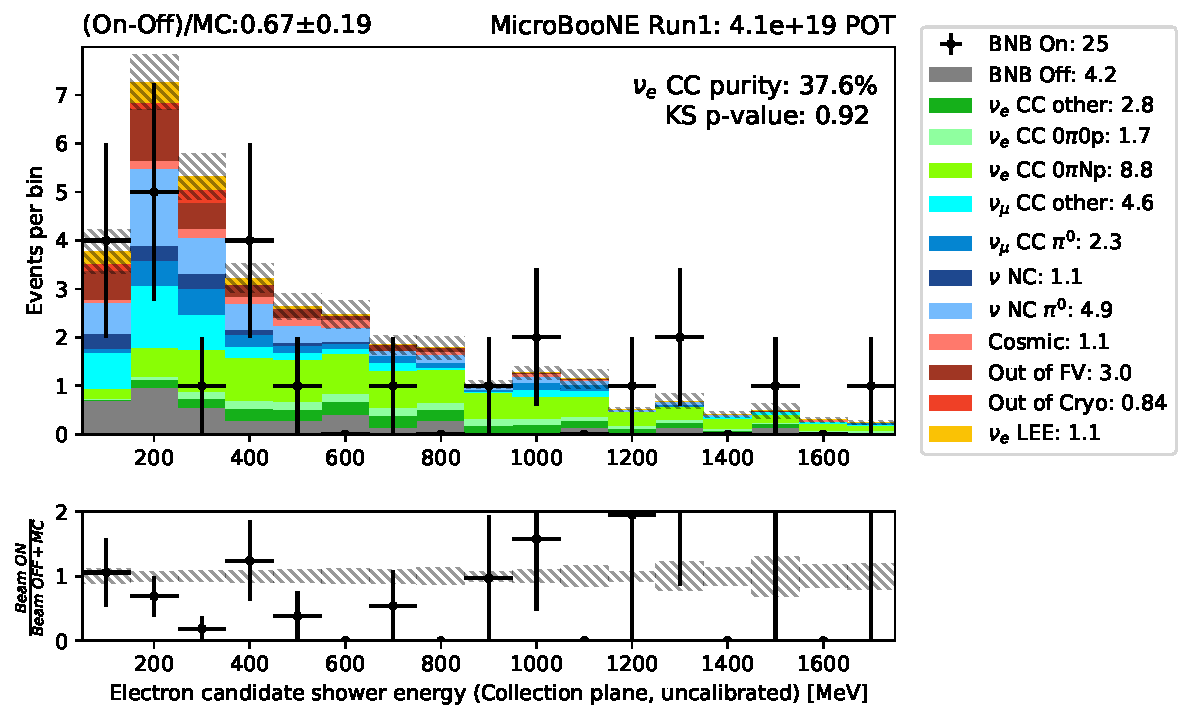
\includegraphics[width=0.545\textwidth]{NueCCsel/Images/run1/nue_shower_energy_y.pdf}
    \caption{(left) BDT response of the $\nu_e$ CC inclusive event classifier. (right) Electron shower energy distribution after the selection.}
    \label{fig:pre_event_score}
\end{figure}

\begin{figure}
    \centering
    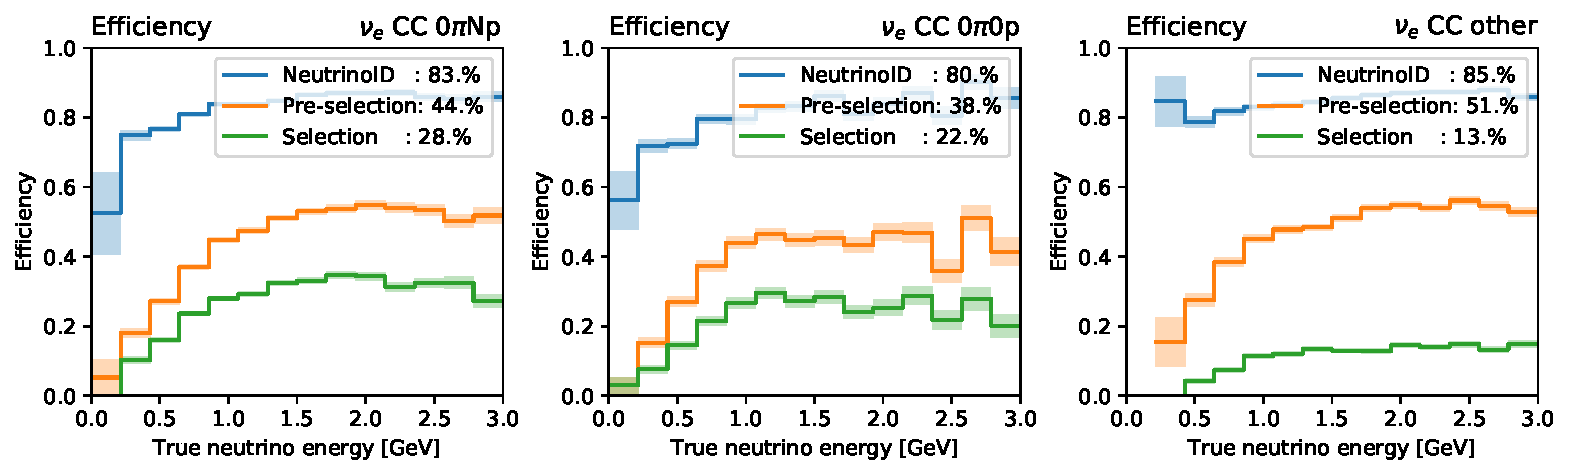
\includegraphics[width=\textwidth]{NueCCsel/Images/run1/efficiency_cat_2.pdf}
    \caption{Efficiency of the different stages in the selection in function of the true neutrino energy. The different panels correspond to different final states of interest.}
    \label{fig:nueccinc_eff}
\end{figure}

